% Created 2018-04-11 mié 19:09
\documentclass[a4paper]{scrartcl}
\usepackage[utf8]{inputenc}
\usepackage[T1]{fontenc}
\usepackage{fixltx2e}
\usepackage{graphicx}
\usepackage{longtable}
\usepackage{float}
\usepackage{wrapfig}
\usepackage{rotating}
\usepackage[normalem]{ulem}
\usepackage{amsmath}
\usepackage{textcomp}
\usepackage{marvosym}
\usepackage{wasysym}
\usepackage{amssymb}
\usepackage{hyperref}
\tolerance=1000
\usepackage{khpreamble}
\usepackage{pgfplots}
\author{Kjartan Halvorsen}
\date{Due Friday 2017-03-15}
\title{Computerized control - homework 4}
\hypersetup{
  pdfkeywords={},
  pdfsubject={},
  pdfcreator={Emacs 24.5.1 (Org mode 8.2.10)}}
\begin{document}

\maketitle

\section*{An observer for the harmonic oscillator model}
\label{sec-1}
The harmonic oscillator model, which in continuous-time has poles in \(\pm i\omega\), can be described in discrete-time as the state-space model
\begin{equation}
\begin{aligned}
x(kh+h) &= \underbrace{\bbm \cos\omega{}h & \frac{1}{\omega} \sin\omega h\\ -\omega\sin\omega h & \cos\omega h\ebm}_{\Phi(h)} x(kh) + \underbrace{\bbm \frac{1}{\omega^2}(1-\cos\omega h)\\\frac{1}{\omega}\sin\omega h\ebm}_{\Gamma(h)} u(kh)\\
y(kh) &= \underbrace{\bbm 1 & 0\ebm}_{C} x(kh)
\end{aligned}
\end{equation}

\begin{enumerate}
\item Determine the eigenvalues of \(\Phi(h)\) (the discrete-time poles of the system). Verify that the poles are the same as obtained through the relationship \(p = \mexp{\lambda h}\) where \(\lambda\) is the continuous-time pole and $p$ is the discrete-time pole.
\item Form the observability matrix \[W_c = \bbm C\\ C\Phi(h) \ebm\] and determine for which values of $h$ the system becomes unobservable.
\item The observer for the system is given by the state-space system
\[ \hat{x}(kh+h) = (\Phi - KC) \hat{x}(kh) + \Gamma(h) u(kh) + Ky(kh) \]
Let \(\omega h = \frac{\pi}{6}\) and determine a gain vector \(K = \bbm k_1 & k_2 \ebm\transp \) that gives a deadbeat observer, i.e. an observer with characteristic polynomial \(z^2\) and poles in the origin.
\end{enumerate}

\section*{Active suspension}
\label{sec-2}
A model of the front suspension of a motorcycle is shown in the figure \ref{fig:quarter}. This model can also be a so-called \emph{quarter model} for the suspension of a car.  The system consists of two masses. The \emph{sprung mass} is the larger of the two masses, and is about half the mass of the motorcyle and rider. The other mass is the much smaller \emph{unsprung mass}, which consists of the mass of the wheel, tyre and part (approximately half) of the suspension system. The two masses are connected by two passive elements: a spring and a damper, as well as an active element: a linear force actuator. The unsprung mass is connected to the ground via a spring representing the tyre (sometimes there is also a damper included in the model of the tyre).
\begin{figure}
\begin{center}
\includegraphics[width=0.65\linewidth]{../figures/active-suspension-nodamper}
\caption{Active suspension model. The heights $h_1(t)$, $h_2(t)$ and $h_g(t)$ are measured with respect to a stationary frame of reference. The vehicle is moving to the right.}
\label{fig:quarter}
\end{center}
\end{figure}

The reference height of the road surface is $h_g = h_0$. When the vehicle is travelling on a horizontal road of this height and the system is in equilibrium, the height of the two masses will be $h_1=h_{1,0}$ and $h_2 = h_{2,0}$, respectively. Introduce deviations from these reference heights
\begin{align*}
h_1(t) &= h_{1,0} + z_1(t)\\
h_2(t) &= h_{2,0} + z_2(t)\\
h_g(t) &= h_{0} + w(t)
\end{align*}

A slightly more complex model is discussed \href{http://ctms.engin.umich.edu/CTMS/index.php?example=Suspension&section=ControlStateSpace}{here}. That model also includes a damping in the tyre. You are welcome to study the example. 

\subsection*{Determine the state space model}
\label{sec-2-1}
There are four forces acting on the sprung mass
\begin{center}
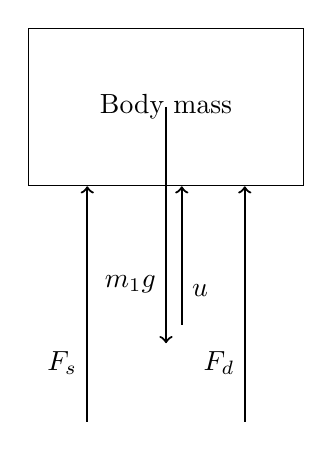
\begin{tikzpicture}
\node (M1) [draw, align=center, minimum width=3.5cm,minimum height=2cm] {Body mass};
\draw[->, thick] (M1.center) -- node[left, near end] {$m_1g$} ++(0, -3cm);
\draw[<-, thick] (M1.south) ++(-1cm, 0) -- node[left, near end] {$F_s$} ++ (0, -3cm);
\draw[<-, thick] (M1.south) ++(1cm, 0) -- node[left, near end] {$F_d$} ++ (0, -3cm);
\draw[<-, thick] (M1.south) ++(0.2cm, 0) -- node[right, near end] {$u$} ++ (0, -1.76cm);
\end{tikzpicture}
\end{center}
The equation of motion in the vertical direction becomes
\begin{equation}
 \begin{split}
 m_1 \ddot{z}_1 &= \sum_i F_i = -m_1g + \underbrace{m_1g -k_1(z_1-z_2)}_{F_s} + \underbrace{\big(-b_1(\dot{z}_1 - \dot{z}_2) \big) }_{F_d} + u  = -k_1(z_1 - z_2) - b_1(\dot{z}_1 - \dot{z}_2) + u\\
                &= -k_1z_1 -b_1\dot{z}_1 + k_1z_2 + b_1\dot{z}_2 + u. 
 \end{split}
 \label{eq:eom1}
 \end{equation}
On the unsprung mass, there are five forces acting:
\begin{center}
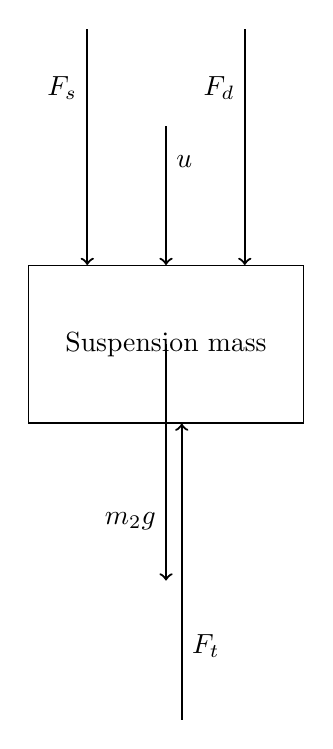
\begin{tikzpicture}
\node (M2) [draw, align=center, minimum width=3.5cm,minimum height=2cm] {Suspension mass};
\draw[->, thick] (M2.center) -- node[left, near end] {$m_2g$} ++(0, -3cm);
\draw[<-, thick] (M2.north) ++(-1cm, 0) -- node[left, near end] {$F_s$} ++ (0, 3cm);
\draw[<-, thick] (M2.north) ++(1cm, 0) -- node[left, near end] {$F_d$} ++ (0, 3cm);
\draw[<-, thick] (M2.north) ++(0cm, 0) -- node[right, near end] {$u$} ++ (0, 1.76cm);
\draw[<-, thick] (M2.south) ++(0.2cm, 0) -- node[right, near end] {$F_t$} ++ (0, -3.76cm);
\end{tikzpicture}
\end{center}
The equation of motion in the vertical direction becomes
\begin{equation}
\begin{split}
m_2\ddot{z}_2 &= -m2_g - \underbrace{\big(m_1g -k_1(z_1-z_2)\big)}_{F_s}
 - \underbrace{\big(- b_1(\dot{z}_1-\dot{z}_2)\big)}_{F_d}
 - \underbrace{\big( (m_1 + m_2)g - k_2(z_2 - w) \big)}_{F_t} - u\\
               &= (k_1)z_1 + b_1\dot{z}_1 - (k_1+k_2)z_2 - b_1\dot{z}_2 + k_2w - u
 \end{split}
 \end{equation}

Use the state-vector     
\[ x = \bbm x_1\\x_2\\x_3\\x_4 \ebm = \bbm z_1\\ \dot{z}_1 \\ z_2\\ \dot{z}_2 \ebm \]
and let the velocity of the sprung mass $y(t) = \dot{z}_1(t)$ be the output of the system. 
\textbf{Set up the continous-time state-space model}
\begin{equation*}
\begin{aligned}
\dot{x}(t) &= Ax(t) + B_u u(t) + B_w w(t)\\
y(t) &= C x(t)
\end{aligned}
\end{equation*}
Note that there are two input signals: The active suspension force $u(t)$ and the disturbance from the road $w(t)$.

\subsection*{Simulate step-responses}
\label{sec-2-2}
Implement the model in matlab. Use the following values for the parameters
\begin{center}
\begin{tabular}{l}
$m1 = 140$\\
$m2 = 14$\\
$k1 = 4.6\cdot{}10^4$\\
$k2 = 3.0\cdot{}10^5$\\
$b1 = 10^3$\\
\end{tabular}
\end{center}
Here is some code to help you
\begin{verbatim}
m1 = 140;
m2 = 14;
k1 = 4.6e4;
k2 = 3.0e5;
b1 = 1e3;

A =   % Your code here

Bu = [0  
     1/m1
     0
     -1/m2 ];
Bw = [ 0
      0
      0
      k2/m2];
C =   % Your code here
D=[0];
sys_uy=ss(A,Bu,C,D); % System with only u(t) as input
sys_wy=ss(A,Bw,C,D); % System with only w(t) as input

% Step responses
figure(1)
clf
subplot(121)
stepplot(1000*sys_uy);
title('Response from u (step 1kN)')
xlabel('Time [s]')
ylabel('y [m/s]')
subplot(122)
stepplot(0.1*sys_wy);
title('Response from w (step 0.1m)')
xlabel('Time [s]')
ylabel('y [m/s]')
\end{verbatim}


\subsection*{Sample the system}
\label{sec-2-3}
\begin{enumerate}
\item The system is quite oscillative, as the step-responses show. Plot the poles of the continuos-time system using \texttt{pzmap} 
\begin{verbatim}
figure(2)
pzmap(sys_uy)
\end{verbatim}
Choose a sampling period $h$, such that $\omega_0h = 0.8$, where $\omega_0$ is the natural frequency (in radians per second) of the fastest poles.
\item Sample the system numerically using \texttt{c2d} in matlab:
\begin{verbatim}
h = % Your code here
sys_uy_d  = c2d(sys_uy, h); % Zero-order-hold sampling
sys_wy_d  = c2d(sys_wy, h); % Zero-order-hold sampling
\end{verbatim}
\end{enumerate}

\subsection*{Determine a state feedback}
\label{sec-2-4}
\begin{enumerate}
\item First determine the desired poles. The system is fourth order, so we need to choose four poles for the closed-loop system. Assume we want the closed-loop system to have more or less the same speed as the two fastest open-loop poles (same distance from the origin), but more damped.  Determine the four desired closed-loop continuous-time poles, and then translate them to discrete time:
\begin{verbatim}
p_c = [ ] % Your four desired closed-loop poles in continuous-time here
p_d = exp(p_c*h) % The corresponding four discrete-time poles
\end{verbatim}
\item Determine the feedback gain vector \(L\), and form the closed-loop system. Matlab will happily do the calculations for you:
\begin{verbatim}
[Phi, Gamma_u, C, D] = ssdata(sys_uy_d) % Get the matrices
[Phi, Gamma_w, C, D] = ssdata(sys_wy_d) 
L = place(Phi, Gamma_u, p_d)    
sys_wy_d_closed = ss(Phi-Gamma_u*L, Gamma_w, C, D, h); % Closed-loop system from w to y
\end{verbatim}
\end{enumerate}

\subsection*{Simulate the closed-loop response}
\label{sec-2-5}
Check the performance of your closed-loop system. Let the disturbance (road profile) look as below
\begin{center}
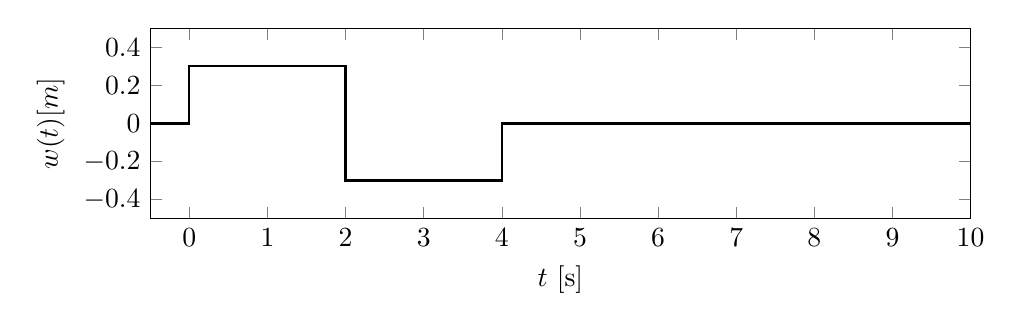
\begin{tikzpicture}
\begin{axis} [
   width = 12cm, height = 4cm,
   xlabel = {$t$ [s]},
   ylabel = {$w(t) [m]$},
   xmin = -0.5, xmax = 10,
   ymin = -0.5, ymax = 0.5,
   ]
   \draw[thick] (axis cs: -0.5,0) -- (axis cs: 0,0) -- (axis cs: 0,0.3) -- (axis cs: 2,0.3) -- (axis cs: 2,-0.3) -- (axis cs: 4,-0.3) -- (axis cs: 4, 0) -- (axis cs: 10,0);
   \end{axis}
   \end{tikzpicture}
   \end{center}

In matlab:
\begin{verbatim}
T = ( 0:ceil(10/h) )*h; % Discrete time-vector from 0 to 10 seconds
w = zeros(size(T));
ind_before_2 = find(T < 2);
w(ind_before_2) = 0.3;
ind_between_2_and_4 = intersect( find(T>2), find(T<4) );
w(ind_between_2_and_4) = -0.3;

[y, Tsim, x] = lsim(sys_wy_d_closed, w, T);
[yo, Tsim, xo] = lsim(sys_wy_d, w, T); % Simulate system without feedback

figure(3)
set(gcf, 'position', [100, 100, 900, 700])
for i=1:4
    subplot(5,1,i)
    stairs(T, x(:,i), 'color', [0, 0.447, 0.741])
    hold on
    stairs(T, xo(:,i), 'color', [0.85, 0.325, 0.098])
    ylabel(sprintf('state %d', i))
    xlabel('Time [s]')
end
legend('Closed-loop response', 'Open-loop response')
subplot(5,1,5)
stairs(T, -L*x', 'color', [0, 0.447, 0.741])
ylabel('Control signal [N]')
\end{verbatim}

\textbf{Comment on the figures!} For instance: How do the closed-loop system response compare to the open-loop response? What was the maximum active suspension force (\(\max u(t)\))? 


\section*{Solutions}
\label{sec-3}

\subsection*{An observer for the harmonic oscillator model}
\label{sec-3-1}
\begin{enumerate}
\item The eigenvalues are given by the roots of \(\det (zI - \Phi)\). Writing \(\cos\omega h = c\) and \(\sin\omega h = s\) for simplicity, we get
\begin{equation*}
\begin{aligned}
\det (zI - \Phi) &= \det \left( \bbm z & 0\\0 & z\ebm - \bbm c & \frac{s}{\omega}\\-\omega s & c\ebm \right) = \det \bbm z-c & -\frac{s}{\omega}\\ \omega s & z-c\ebm \\
&= (z-c)^2 + s^2
\end{aligned}
\end{equation}
with roots on the unit circle:
\[ z = c \pm is = \cos\omega h \pm i \sin\omega h.\]
Using the relationship \(z = \mexp{sh}\) between the s-plane and the z-plane we get for the continous-time poles \(s=\pm i\omega\)
\[ z = \mexp{\pm i\omega h} = \cos\omega h \pm i\sin\omega h \]
using Euler's formula.
\item The observability matrix becomes
\[ W_c = \bbm C\\C\Phi \ebm = \bbm 1 & 0\\ c & \frac{s}{\omega},\] so
\[ \det W_c = \frac{1}{\omega} \sin\omega h \]
which is zero for \(\omega h = k\pi, \; k=1,2,\ldots\). So observability is lost for
\[ h = \frac{k\pi}{\omega}, \; k=1,2\ldots. \]
\item With \(\omega=1\) and \(h=\frac{\pi}{6}\) we get \(\cos\omega h = \sqrt{3}/2\) and \(\sin\omega h = 1/2\). This gives
\end{enumerate}
\[ \Phi = \frac{1}{2} \bbm \sqrt{3} & 1\\-1 & \sqrt{3} \ebm\].
The characteristic polynomial of the observer becomes
\begin{equation*}
\begin{aligned}
\det \big(zI - (\Phi - KC)\) &= \det  \left( \bbm z & 0\\0 & z\ebm - \frac{1}{2} \bbm \sqrt{3} - 2k_1 & 1\\-1-2k_2 & \sqrt{3}\ebm\\
&= \det \bbm z-\frac{\sqrt{3}-2k_1}{2} & -\frac{1}{2}\\\frac{1+2k_2}{2} & z - \frac{\sqrt{3}}{2} \ebm\\
&= (z-\frac{\sqrt{3}-2k_1}{2})(z - \frac{\sqrt{3}}{2}) + \frac{1+2k_2}{4}\\
&= z^2 - (\sqrt{3}-k_1)z + \frac{1}{4}\big( \sqrt{3}(\sqrt{3}-2k_1) + 1 + 2k_2\big)\\
&= z^2 - (\sqrt{3}-k_1)z + \frac{1}{4}\big(-2\sqrt{3}k_1 + 2k_2 + 4\big)
\end{aligned}
\end{equation*}
Setting coefficient equal to the coefficients of the desired characteristic polynomial \(z^2\) gies
\begin{align*}
\sqrt{3}-k_1 &= 0 \quad \Rightarrow \quad k_1 = \sqrt{3}\\
-2\sqrt{3}k_1 + 2k_2 + 4 &= 0 \quad \Rightarrow \quad k_2 = 3-2 = 1
\end{align*}

\subsection*{Active suspension}
\label{sec-3-2}
\subsubsection*{State space model}
\label{sec-3-2-1}
With the state vector 
 \[ x = \bbm x_1\\x_2\\x_3\\x_4 \ebm = \bbm z_1\\ \dot{z}_1 \\ z_2\\ \dot{z}_2 \ebm \]
 we can write the four first-order differential equations of the state space model
 \begin{align*}
  \dot{x}_1 &= \dot{z}_1 = x_2\\
  \dot{x}_2 &= \ddot{z}_1 = \frac{1}{m_1}\Big(-k_1z_1 -b_1\dot{z}_1 + k_1z_2 + b_1\dot{z}_2 + u\Big)\\
            &= -\frac{k_1}{m_1}x_1 - \frac{b_1}{m_1}x_2 + \frac{k_1}{m_1}x_3 + \frac{b_1}{m_2}x_4 + \frac{1}{m_1} u\\
  \dot{x}_3 &= \dot{z}_2 = x_4\\
  \dot{x}_4 &= \ddot{z}_2 = \frac{1}{m_2} \Big(k_1z_1 + b_1\dot{z}_1 - (k_1+k_2)z_2 - b_1\dot{z}_2 + k_2w - u\Big)\\ 
            &= \frac{k_1}{m_2} x_1 + \frac{b_1}{m_2} x_2 - \frac{k_1+k_2}{m_2}x_3 + -\frac{b_1}{m_2}x_4 + \frac{k_2}{m_2}w - \frac{1}{m_2}u.
\end{align*}
In state-space form, this can be written
\begin{align*}
\dot{x} &= \bbm 0 & 1 & 0 & 0\\ 
-\frac{k_1}{m_1} & -\frac{b_1}{m_1} & \frac{k_1}{m_1} & \frac{b_1}{m_1}\\
0 & 0 & 0 & 1\\
\frac{k_1}{m_2} & \frac{b_1}{m_2} & -\frac{k_1+k_2}{m_2} & -\frac{b_1}{m_2}\ebm
\bbm x_1\\x_2\\x_3\\x_4 \ebm + \bbm 0\\0\\0\\\frac{k_2}{m_2} \ebm w + \bbm 0\\\frac{1}{m_1}\\0\\-\frac{1}{m_2} \ebm u \\
y &= \bbm 0 & 1 & 0 & 0 \ebm x.
\end{align*}

\subsubsection*{step-responses}
\label{sec-3-2-2}
The figure below shows the step-responses of both the continuous- and the sampled systems.
\begin{center}
\includegraphics[width=0.6\linewidth]{active-susp-plant-response}
\end{center}

\subsubsection*{Sampling the system}
\label{sec-3-2-3}
\begin{enumerate}
\item The pole-zero map below shows that the fast poles have a distance of \(\omega = 156\) rad/s to the origin. The rule-of-thumb (chapter 2.9 in the textbook) tells us that we should have \(\omega h \approx 0.2 -- 0.6\). For instance,
\[ h = \frac{0.6}{156} \approx \unit{0.004}{\second}. \]
\item Sampling the system is straightforward 
\begin{verbatim}
h = 0.004;
sys_uy_d = c2d(sys_uy, h); % The system from input u to y
sys_wy_d = c2d(sys_wy, h); % From input w to y
\end{verbatim}
\end{enumerate}
\subsubsection*{State feedback}
\label{sec-3-2-4}
\begin{enumerate}
\item Desired closed-loop poles. The idea is to choose the poles to be equally fast, but more damped than the fast poles of the plant. For instance we can choose the set of four poles  
\[ p_{1,2} = -\zeta_1\omega_n \pm i \sqrt{1 - \zeta_1^2}\omega_n,  \quad
               p_{3,4} = -\zeta_2\omega_n \pm i \sqrt{1 - \zeta_2^2}\omega_n \]
with natural frequency \(\omega_n = 156\), and damping ratio \(\zeta_1 = 0.8\) and \(\zeta_2 = 0.6\).
\item The feedback vector is calculated by Matlab and gives
$\backslash$[ L = \bbm l$_{\text{1}}$ \& l$_{\text{2}}$ \& l$_{\text{3}}$ \& l$_{\text{4}}$ \ebm = \bbm 1.89$\cdot$ 10$^{\text{6}}$ \& 3.85 $\cdot$ 10$^{\text{4}}$ \& -3.23$\cdot$ 10$^{\text{5}}$ \& 6.20 $\cdot$ 10$^{\text{2}\ebm}$.
\end{enumerate}

\subsubsection*{Simulations}
\label{sec-3-2-5}
With the state feedback proposed, the response is as shown in the figure below.
\begin{center}
\includegraphics[width=\linewidth]{../matlab/active-suspension-sim-crop}
\end{center}
We can see that the closed-loop response of \(z_1\) and \(\dot{z}_1\) are both very well damped, and has much smaller amplitude than the open-loop system. The control signal shows quite large peak (30-50 kN) at the onset of the disturbances. 

\subsubsection*{Choosing the closed-loop poles too slow.}
\label{sec-3-2-6}
There is a potential problem with choosing the closed-loop poles (much) slower than the open-loop poles in this exercise. Slow poles in discrete-time means close to 1. The reason is that state feedback does not change the numerator in the pulse transfer function from input to output.  So, if the open-loop pulse transfer function from disturbance to output signal is
\[ H_w(z) = C (zI-\Phi)^{-1} \Gamma_w = \frac{\beta(z)}{\alpha(z)},\]
then the closed-loop transfer function will be 
\[ H_c(z) = C \big(zI -(\Phi-\Gamma_u L)\big)^{-1}\Gamma_w = \frac{\beta(z)}{\alpha_c(z)}.\]
The denominator is obtained by design (choice of pole placement) to have the roots (desired closed-loop poles) \(p_{d,1}\),  \(p_{d,2}\),  \(p_{d,3}\),  \(p_{d,4}\), so   
\[ H_c(z) = \frac{\beta(z)}{(z-p_{d,1})(z-p_{d,2})(z-p_{d,3})(z-p_{d,4})}.\]
The static gain becomes
\[ H_c(1) = \frac{\beta(1)}{(1-p_{d,1})(1-p_{d,2})(1-p_{d,3})(1-p_{d,4})},\]
which can be much larger than the open-loop static gain \(H_w(1)\), if the closed-loop poles are much closer to 1 than the open-loop poles. 
% Emacs 24.5.1 (Org mode 8.2.10)
\end{document}